\section{Experiment design}\label{sec:experiment_design}
%Forsoegsopstilling, der inkludere en tegning af omraadet set oppefra med indtegning af beacons, objectern og hvor rigtige position for test person.
The implemented system's evaluation experiments are conducted in a room measuring $4.75m \times 6.5m$.
In the room, a cabinet is placed between two tables, effectively dividing the room into two smaller areas. 
Each of the smaller areas are furnished with a table surrounded by six chairs, and whiteboards mounted on the walls.
\begin{figure}[h!]
    \centering
    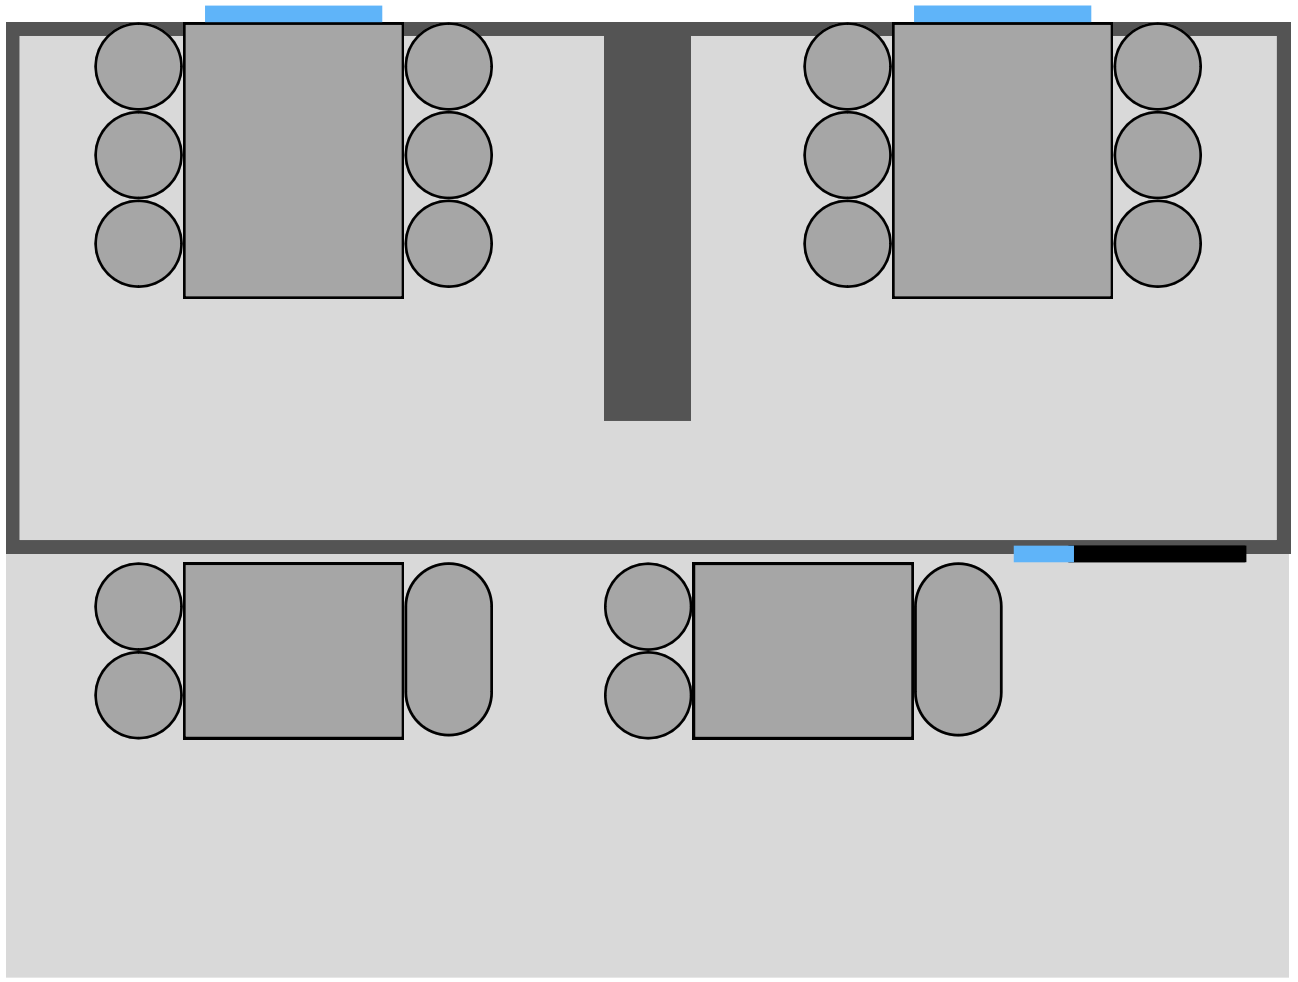
\includegraphics[scale=0.5]{images/experiment_room.png}
    \caption{A sketch of the meeting room in which the experiments were carried out.}
    \label{fig:experiment_room}
\end{figure}
On one end of each table is a large, rectangular window.
Furthermore, one table has a large TV screen placed near its window. 
Near the door of the room, an airconditioning controller and a large glass pane, acting as a window out into the common area, is located. 
Next to the door is placed a glass pane, acting as a window out into the common area. 
Lighting is built into the ceiling, thus no hanging light will interfere with the broadcasted signals. 
Outside the meeting room, is the aforementioned common area containing two high tables.
Each of these tables has a small couch and two chairs placed next to it.
The meeting room and its surrounding area is depicted in Figure \ref{fig:experiment_room}.

Four Bluetooth iBeacon BLE9 beacons \cite{BluetoothiBeaconBLE9} are placed on top of the cabinet and in the three corners furthest away from the door. 
The beacons in the corners of the room are placed in a height of $2.5m$, while the center beacon on top of the cabinet is placed in a height of $1.5m$.   
The beacons placed near the windows are located on top of a whiteboard, while the beacon in the lower left corner of the room is held in place using painter's tape. 

%Mention the threshold and argue why its set to .5

%Explain the configuration of the grid


